\documentclass[10pt,a4paper]{article}

% --- Package Imports ---
\usepackage[utf8]{inputenc}
\usepackage[T1]{fontenc}
\usepackage{helvet}
\renewcommand{\familydefault}{\sfdefault}
\usepackage{microtype}

\usepackage[margin=0.75in,top=0.85in,bottom=0.85in]{geometry}
\usepackage{amsmath,amssymb}
\usepackage{xcolor}
\usepackage{colortbl}
\usepackage{booktabs}
\usepackage{tabularx}
\usepackage{enumitem}
\usepackage{fancyhdr}
\usepackage{titlesec}
\usepackage{fontawesome5}
\usepackage[most]{tcolorbox}
\usepackage{tikz}
\usetikzlibrary{positioning,calc,shapes.geometric,backgrounds}

% --- Color Palette Definition ---
% Tasteful 4-color professional palette
\definecolor{NavyPrimary}{HTML}{1E293B}     % Deep Slate Navy for headers and text
\definecolor{TealAccent}{HTML}{0F766E}      % Elegant Dark Teal for accents
\definecolor{TealLight}{HTML}{F0FDFA}       % Soft Teal Tint for highlights/boxes
\definecolor{SlateLight}{HTML}{F8FAFC}      % Clean light background fill
\definecolor{BorderGray}{HTML}{CBD5E1}      % Subtle gray border
\definecolor{AmberWarn}{HTML}{D97706}       % Warm Amber for growth recommendations
\definecolor{GreenPass}{HTML}{166534}       % Deep Forest Green for strengths
\definecolor{TextDark}{HTML}{334155}        % Primary body text
\definecolor{TextMuted}{HTML}{64748B}       % Subtitle/secondary text

% --- Page Style Setup ---
\pagestyle{fancy}
\fancyhf{}
\renewcommand{\headrulewidth}{0pt}
\renewcommand{\footrulewidth}{0.5pt}
\renewcommand{\footrule}{\color{BorderGray}\hrule width\headwidth height\footrulewidth}

\lfoot{\small\color{TextMuted}\faGraduationCap\ \ Meridian University --- Faculty Development \& Assessment Center}
\cfoot{\small\color{TextMuted}Peer Classroom Evaluation Report}
\rfoot{\small\color{TextMuted}Page \thepage\ of 3}

% --- Section Styling ---
\titleformat{\section}
  {\color{NavyPrimary}\Large\bfseries}
  {\thesection.}{0.5em}{}
  [\color{TealAccent}\titlerule]

\titleformat{\subsection}
  {\color{TealAccent}\large\bfseries}
  {\thesubsection}{0.5em}{}

\titlespacing*{\section}{0pt}{14pt}{8pt}
\titlespacing*{\subsection}{0pt}{10pt}{4pt}

% --- Custom tcolorbox Styles ---
\tcbset{
  basebox/.style={
    enhanced,
    arc=4pt,
    boxrule=0.8pt,
    left=10pt,right=10pt,top=8pt,bottom=8pt,
    fonttitle=\bfseries\color{white},
  }
}

\newtcolorbox{headerbox}{
  enhanced,
  colback=NavyPrimary,
  colframe=NavyPrimary,
  arc=6pt,
  left=14pt, right=14pt, top=12pt, bottom=12pt,
  shadow={2pt}{-2pt}{0pt}{black!20}
}

\newtcolorbox{infocard}[1][]{
  enhanced,
  colback=SlateLight,
  colframe=BorderGray,
  arc=4pt,
  boxrule=0.6pt,
  left=10pt, right=10pt, top=8pt, bottom=8pt,
  #1
}

\newtcolorbox{scorebox}[1]{
  enhanced,
  colback=TealLight,
  colframe=TealAccent,
  arc=4pt,
  boxrule=1pt,
  title=#1,
  coltitle=white,
  left=8pt, right=8pt, top=6pt, bottom=6pt
}

\newtcolorbox{strengthbox}{
  enhanced,
  colback=GreenPass!10!white,
  colframe=GreenPass,
  arc=4pt,
  boxrule=0.8pt,
  title={\faCheckCircle\ \ Primary Observed Strengths},
  coltitle=white,
  left=10pt, right=10pt, top=8pt, bottom=8pt
}

\newtcolorbox{growthbox}{
  enhanced,
  colback=AmberWarn!10!white,
  colframe=AmberWarn,
  arc=4pt,
  boxrule=0.8pt,
  title={\faExclamationTriangle\ \ Areas for Growth \& Development},
  coltitle=white,
  left=10pt, right=10pt, top=8pt, bottom=8pt
}

% --- Custom Rating Scale Helper ---
\newcommand{\ratingstars}[1]{%
  \begin{tikzpicture}[baseline=-0.5ex, scale=0.85]
    \foreach \i in {1,...,5} {
      \ifnum \i > #1 \relax
        \node[inner sep=0pt] at (\i*0.35,0) {\color{BorderGray}\faStar};
      \else
        \node[inner sep=0pt] at (\i*0.35,0) {\color{AmberWarn}\faStar};
      \fi
    }
  \end{tikzpicture}%
}

\begin{document}

% ==========================================
% PAGE 1: HEADER & EVALUATION METADATA
% ==========================================

\begin{headerbox}
  \begin{minipage}[c]{0.70\textwidth}
    {\color{white}\huge\bfseries MERIDIAN UNIVERSITY}\\[3pt]
    {\color{TealLight}\large\bfseries Office of Academic Excellence \& Faculty Advancement}\\[2pt]
    {\color{white}\small Formal Peer Classroom Observation \& Evaluation Report}
  \end{minipage}%
  \hfill
  \begin{minipage}[c]{0.26\textwidth}
    \raggedleft
    
\begin{tikzpicture}
      \node[draw=TealLight, fill=TealAccent, rounded corners=4pt, inner sep=6pt, text=white, align=center] {
        \footnotesize\textbf{CONFIDENTIAL}\\[1pt]
        \scriptsize Faculty Peer Review\\
        \scriptsize AY 2025--2026
      };
    \end{tikzpicture}
  \end{minipage}
\end{headerbox}

\vspace{8pt}

% Section 1: Overview & Metadata
\begin{infocard}
  \begin{tabularx}{\textwidth}{@{}l X l X@{}}
    \textbf{\color{NavyPrimary}Instructor Evaluated:} & Dr. Eleanor Vance & \textbf{\color{NavyPrimary}Evaluation Date:} & October 14, 2025 \\
    \textbf{\color{NavyPrimary}Academic Title:} & Associate Professor & \textbf{\color{NavyPrimary}Observation Time:} & 10:00 AM -- 11:30 AM \\
    \textbf{\color{NavyPrimary}Department:} & Computer Science \& Engineering & \textbf{\color{NavyPrimary}Location / Room:} & Turing Hall, Room 204 \\
    \textbf{\color{NavyPrimary}Course Code \& Name:} & CS 342: Algorithms \& Data Structures & \textbf{\color{NavyPrimary}Students Present:} & 42 / 45 Enrolled (93\%) \\
    \textbf{\color{NavyPrimary}Peer Observer:} & Prof. Marcus Holloway (Dept. Chair) & \textbf{\color{NavyPrimary}Session Topic:} & Graph Algorithms: Dijkstra \& Heaps \\
  \end{tabularx}
\end{infocard}

\vspace{10pt}

% Executive Summary Score Card
\begin{minipage}[t]{0.31\textwidth}
  \begin{scorebox}{Overall Performance Rating}
    \centering
    \vspace{2pt}
    {\color{NavyPrimary}\Huge\bfseries 4.85 \Large/ 5.0}\\[4pt]
    \ratingstars{5}\\[4pt]
    {\color{TealAccent}\bfseries\small Exemplary Performance}\\
    \scriptsize Exceeds departmental standards across all major evaluated metrics.
  \end{scorebox}
\end{minipage}%
\hfill
\begin{minipage}[t]{0.66\textwidth}
  \begin{infocard}[title={\textbf{\color{NavyPrimary}\faFile\ Executive Summary}}, colback=white, colframe=NavyPrimary]
    Dr. Vance demonstrated outstanding pedagogical clarity and classroom leadership during the 90-minute lecture on graph traversal and shortest-path optimization. The session combined rigorous theoretical foundations with interactive live-coding demonstrations and structured peer discussion. Students exhibited exceptionally high engagement, asking insightful questions that were adeptly integrated into the core lesson plan.
  \end{infocard}
\end{minipage}

\vspace{12pt}

% Section 2: Detailed Observation Rubric
\section{Detailed Classroom Observation Rubric}

\begin{tcolorbox}[colback=white, colframe=NavyPrimary, arc=4pt, boxrule=0.8pt, left=4pt, right=4pt, top=4pt, bottom=4pt]
\small
\begin{tabularx}{\textwidth}{@{} >{\bfseries\color{NavyPrimary}}p{3.2cm} X c >{\centering\arraybackslash}p{2.8cm} @{}}
\rowcolor{NavyPrimary}
\color{white}Domain / Metric & \color{white}Specific Evaluation Criteria & \color{white}Score & \color{white}Rating Level \\
\midrule

\multicolumn{4}{@{}l@{}}{\cellcolor{TealLight}\textbf{\color{TealAccent}\faBook\ Part 1: Instructional Design \& Content Mastery}} \\
\midrule

1.1 Learning Objectives & Clear, explicit statement of session goals connected to prior course modules and upcoming assignments. & 5.0 / 5 & Exemplary \\
1.2 Subject Mastery & Thorough, confident command of algorithm complexity, edge-case analysis, and data structure tradeoffs. & 5.0 / 5 & Exemplary \\
1.3 Structural Pacing & Logical progression from concept review to live pseudocode analysis and complexity proof. & 4.7 / 5 & High Proficiency \\
1.4 Clarity \& Presentation & Precise verbal explanations, excellent whiteboard organization, and effective visual diagrams. & 4.9 / 5 & Exemplary \\

\midrule
\multicolumn{4}{@{}l@{}}{\cellcolor{TealLight}\textbf{\color{TealAccent}\faUsers\ Part 2: Pedagogical Execution \& Classroom Atmosphere}} \\
\midrule

2.1 Student Engagement & Proactively solicits input from diverse sections of the lecture hall; encourages student inquiry. & 4.8 / 5 & Exemplary \\
2.2 Question Handling & Validates student questions, redirects inquiries to test class comprehension, and clarifies misconceptions. & 5.0 / 5 & Exemplary \\
2.3 Educational Tech & Seamless integration of tablet annotations, IDE code execution, and dynamic graph visualizations. & 4.6 / 5 & High Proficiency \\
2.4 Inclusivity \& Climate & Fosters a respectful, encouraging learning environment where students comfortably share partial solutions. & 5.0 / 5 & Exemplary \\

\bottomrule
\end{tabularx}
\end{tcolorbox}

\vfill
\centerline{\small\color{TextMuted}\textit{Continued on next page --- Part 3 \& Narrative Qualitative Feedback}}
\newpage

% ==========================================
% PAGE 2: NARRATIVE EVALUATION & STRENGTHS
% ==========================================

\section{Detailed Observation Notes \& Narrative Analysis}

\subsection{1. Domain-Specific Pedagogical Strengths}

Dr. Vance's instructional delivery represents a masterclass in computer science education. The following key observations were recorded during the 90-minute evaluation:

\begin{enumerate}[label=\textbf{\color{TealAccent}\lbrack\arabic*\rbrack}, leftmargin=*]
  \item \textbf{Dual-Channel Information Delivery:} Dr. Vance effectively paired theoretical proof work on the primary whiteboard with live algorithm tracing on a digitized tablet display. This allowed students to visualize both mathematical guarantees and practical data structure mutations concurrently.
  \item \textbf{Active Retrieval Practice:} At minute 25, Dr. Vance paused the lecture to launch a 4-minute pair-think-share exercise on heap operations. This technique successfully re-engaged the room and allowed her to gauge comprehension before transitioning to complex shortest-path edge cases.
  \item \textbf{Scaffolded Questioning Techniques:} When a student posed a question regarding negative edge weights in Dijkstra's algorithm, Dr. Vance guided the student to discover the failure condition independently through targeted, incremental prompts rather than simply supplying the answer.
\end{enumerate}

\vspace{8pt}

\begin{minipage}[t]{0.48\textwidth}
  \begin{strengthbox}
    \small
    \begin{itemize}[leftmargin=12pt, label={\color{GreenPass}\faCheck}]
      \item Exceptional clarity in explaining algorithmic time complexity ($\mathcal{O}((V + E) \log V)$).
      \item Outstanding classroom presence and vocal modulation.
      \item Smooth transition between high-level theory and implementation details.
      \item Highly effective use of real-time polling to identify student misconceptions.
    \end{itemize}
  \end{strengthbox}
\end{minipage}%
\hfill
\begin{minipage}[t]{0.48\textwidth}
  \begin{growthbox}
    \small
    \begin{itemize}[leftmargin=12pt, label={\color{AmberWarn}\faExclamation}]
      \item \textbf{Board Space Management:} The lower right panel of the whiteboard became cluttered during the final 10 minutes.
      \item \textbf{Time Allocation:} The final wrap-up summary was slightly rushed due to extended student discussion on priority queues.
      \item \textbf{Microphone Audio:} Minor volume drop when writing on the board away from the podium mic.
    \end{itemize}
  \end{growthbox}
\end{minipage}

\vspace{14pt}

\subsection{2. Quantitative Scoring Breakdown by Category}

The chart below illustrates the peer evaluation scores across the four core dimensions assessed by the Faculty Evaluation Committee.

\vspace{6pt}

\begin{center}
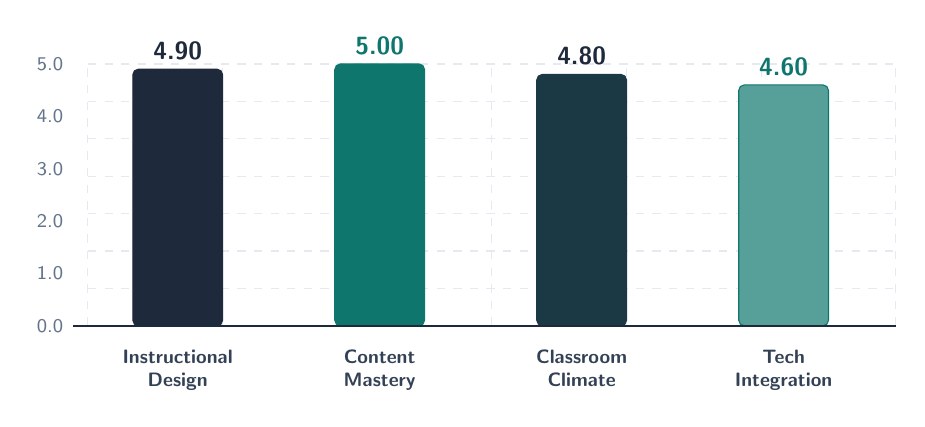
\begin{tikzpicture}[scale=0.95]
  % Grid lines
  \draw[color=BorderGray!50, dashed] (0,0) grid[ystep=0.5cm, xstep=1.8cm] (10.8,3.5);
  
  % Y Axis Labels
  \foreach \y/\val in {0/0.0, 0.7/1.0, 1.4/2.0, 2.1/3.0, 2.8/4.0, 3.5/5.0} {
    \node[anchor=east, font=\scriptsize\color{TextMuted}] at (-0.2, \y) {\val};
  }
  
  % X Axis Bars
  % Bar 1: Course Design (4.9)
  \draw[fill=NavyPrimary, draw=NavyPrimary, rounded corners=2pt] (0.6,0) rectangle (1.8, 3.43);
  \node[above, font=\bfseries\small\color{NavyPrimary}] at (1.2, 3.43) {4.90};
  \node[below, font=\scriptsize\bfseries\color{TextDark}, align=center] at (1.2, -0.2) {Instructional\\Design};
  
  % Bar 2: Subject Mastery (5.0)
  \draw[fill=TealAccent, draw=TealAccent, rounded corners=2pt] (3.3,0) rectangle (4.5, 3.5);
  \node[above, font=\bfseries\small\color{TealAccent}] at (3.9, 3.5) {5.00};
  \node[below, font=\scriptsize\bfseries\color{TextDark}, align=center] at (3.9, -0.2) {Content\\Mastery};
  
  % Bar 3: Classroom Climate (4.8)
  \draw[fill=NavyPrimary!80!TealAccent, draw=NavyPrimary!80!TealAccent, rounded corners=2pt] (6.0,0) rectangle (7.2, 3.36);
  \node[above, font=\bfseries\small\color{NavyPrimary}] at (6.6, 3.36) {4.80};
  \node[below, font=\scriptsize\bfseries\color{TextDark}, align=center] at (6.6, -0.2) {Classroom\\Climate};
  
  % Bar 4: Tech Integration (4.6)
  \draw[fill=TealAccent!70!white, draw=TealAccent, rounded corners=2pt] (8.7,0) rectangle (9.9, 3.22);
  \node[above, font=\bfseries\small\color{TealAccent}] at (9.3, 3.22) {4.60};
  \node[below, font=\scriptsize\bfseries\color{TextDark}, align=center] at (9.3, -0.2) {Tech\\Integration};

  % Baseline
  \draw[thick, color=NavyPrimary] (-0.2,0) -- (10.8,0);
\end{tikzpicture}
\end{center}

\vspace{10pt}

\subsection{3. Student Engagement \& Inclusivity Assessment}

Observation confirmed that Dr. Vance creates an equitable and supportive atmosphere. Student participation was balanced across gender and seating rows. Of the 18 individual student contributions logged during the lecture:
\begin{itemize}[label=\textcolor{TealAccent}{\small\faCircle}, leftmargin=18pt]
  \item \textbf{11 responses} were student-initiated inquiries seeking deeper clarification on algorithm mechanics.
  \item \textbf{7 responses} were answers to instructor-prompted checking questions.
  \item Dr. Vance consistently validated all attempts before building upon them, reinforcing a growth-mindset environment.
\end{itemize}

\vfill
\centerline{\small\color{TextMuted}\textit{Continued on next page --- Post-Observation Action Plan \& Formal Signatures}}
\newpage

% ==========================================
% PAGE 3: ACTION PLAN & SIGN-OFF
% ==========================================

\section{Post-Observation Conference \& Action Plan}

Following the classroom observation, Dr. Vance and Prof. Holloway met for a 45-minute debrief on October 16, 2025. The following mutually agreed-upon goals were established for further professional development:

\vspace{6pt}

\begin{tcolorbox}[colback=SlateLight, colframe=NavyPrimary, title={\textbf{\color{white}\faTasks\ Post-Observation Action Plan (AY 2025--2026)}}, arc=4pt]
\small
\begin{tabularx}{\textwidth}{@{} c X p{3.2cm} p{2.8cm} @{}}
\rowcolor{TealLight}
\textbf{\color{TealAccent}\#} & \textbf{\color{TealAccent}Action Item / Growth Objective} & \textbf{\color{TealAccent}Support / Resource} & \textbf{\color{TealAccent}Target Date} \\
\midrule

\textbf{1} & \textbf{Lavalier Lapel Microphone Adoption:} Utilise wireless lapel mic to ensure consistent audio fidelity when moving across the lecture stage. & Campus AV Services & Immediate \\
\addlinespace[4pt]

\textbf{2} & \textbf{Board Layout Pre-Structuring:} Reserve the far-left panel strictly for persistent definitions and key notation to avoid end-of-class crowding. & Self-implementation & Next Module (Nov 2025) \\
\addlinespace[4pt]

\textbf{3} & \textbf{Peer Faculty Seminar Presentation:} Share active retrieval techniques and pair-think-share models with junior department faculty. & Center for Teaching Excellence & Spring 2026 Seminar \\

\bottomrule
\end{tabularx}
\end{tcolorbox}

\vspace{14pt}

\section{Evaluator Recommendations \& Summary Statement}

\begin{infocard}[colback=white, colframe=TealAccent, boxrule=1pt]
\small\color{TextDark}
\textbf{Recommendation for Reappointment / Promotion Status:} \textcolor{GreenPass}{\textbf{STRONGLY RECOMMENDED}}\\[4pt]
Dr. Eleanor Vance continues to exemplify high-impact university teaching. Her mastery of complex computer science pedagogy, combined with genuine enthusiasm and structured student engagement, places her among the top educators in the department. The minor recommendations noted above reflect opportunities for fine-tuning an already exceptional classroom methodology.
\end{infocard}

\vspace{24pt}

% Section 5: Signatures \& Formal Verification
\section{Formal Sign-off \& Acknowledgments}

By signing below, the evaluator and instructor acknowledge that the peer observation was conducted in accordance with Meridian University Faculty Handbook Section 4.2 (Peer Review Guidelines), and that a post-observation debrief was completed.

\vspace{20pt}

\begin{minipage}[t]{0.45\textwidth}
  \color{NavyPrimary}
  \rule{\textwidth}{0.6pt}\\[4pt]
  \textbf{Prof. Marcus Holloway}\\
  \small Peer Observer / Department Chair\\
  \scriptsize Department of Computer Science \& Engineering\\
  \scriptsize Date: October 17, 2025
\end{minipage}%
\hfill
\begin{minipage}[t]{0.45\textwidth}
  \color{NavyPrimary}
  \rule{\textwidth}{0.6pt}\\[4pt]
  \textbf{Dr. Eleanor Vance}\\
  \small Evaluated Faculty Member\\
  \scriptsize Associate Professor of Computer Science\\
  \scriptsize Date: October 17, 2025
\end{minipage}

\vspace{35pt}

\begin{minipage}[t]{0.45\textwidth}
  \color{NavyPrimary}
  \rule{\textwidth}{0.6pt}\\[4pt]
  \textbf{Dr. Harrison Sterling}\\
  \small Dean, College of Engineering \& Information Technology\\
  \scriptsize Meridian University\\
  \scriptsize Date: October 20, 2025
\end{minipage}%
\hfill
\begin{minipage}[t]{0.45\textwidth}
  
\begin{tikzpicture}
    \node[draw=BorderGray, fill=SlateLight, rounded corners=4pt, inner sep=8pt, text width=0.42\textwidth, align=center] {
      \color{NavyPrimary}\small\bfseries Institutional Assessment Seal\\[2pt]
      \color{TextMuted}\tiny Form Ref: MU-PEER-2025-CS342\\[1pt]
      \color{TextMuted}\tiny Archived in Faculty Performance Record
    };
  \end{tikzpicture}
\end{minipage}

\end{document}

